\message{ !name(oldpaper.tex)}\documentclass[10pt,twocolumn,letterpaper]{article}

\usepackage{cvpr} \usepackage{times} \usepackage{epsfig}
\usepackage{graphicx} \usepackage{amsmath} \usepackage{amssymb}
\usepackage{subfig}

% Include other packages here, before hyperref.

% If you comment hyperref and then uncomment it, you should delete
% egpaper.aux before re-running latex.  (Or just hit 'q' on the first
% latex run, let it finish, and you should be clear).
\usepackage[pagebackref=true,breaklinks=true,letterpaper=true,colorlinks,bookmarks=false]{hyperref}


 \cvprfinalcopy % *** Uncomment this line for the final submission

\def\cvprPaperID{84} % *** Enter the 3DIMPVT Paper ID here
\def\httilde{\mbox{\tt\raisebox{-.5ex}{\symbol{126}}}}

% Pages are numbered in submission mode, and unnumbered in
% camera-ready
\ifcvprfinal\pagestyle{empty}\fi
\begin{document}

\message{ !name(oldpaper.tex) !offset(667) }
\section{Results and Conclusions}
\label{sec:resultsAndConclusions}
Examples of ceilings and floors textured with the tile caching
approach, and walls textured with the seam minimization approach, are
displayed in Figure \ref{fig:results}. High resolution texture
comparisons, as well as a walkthrough of a fully textured 3D model are
available in the accompanying video to this paper.

In this paper, we have developed an approach to texture map models
with noisy camera localization data. We are able to refine image
locations based on feature matching, and robustly handle outliers. The
tile-based mapping approach can be used to texture both simple
rectangular walls as well as complex floor and ceiling geometry. We
also presented a seam minimization texturing method that produces
seamless textures on planes where multiple head-on images are
available. Each of these approaches is highly modular, and easily
tunable for different environments and acquisition hardware.




\begin{figure*}
  \centering
  \subfloat[][]{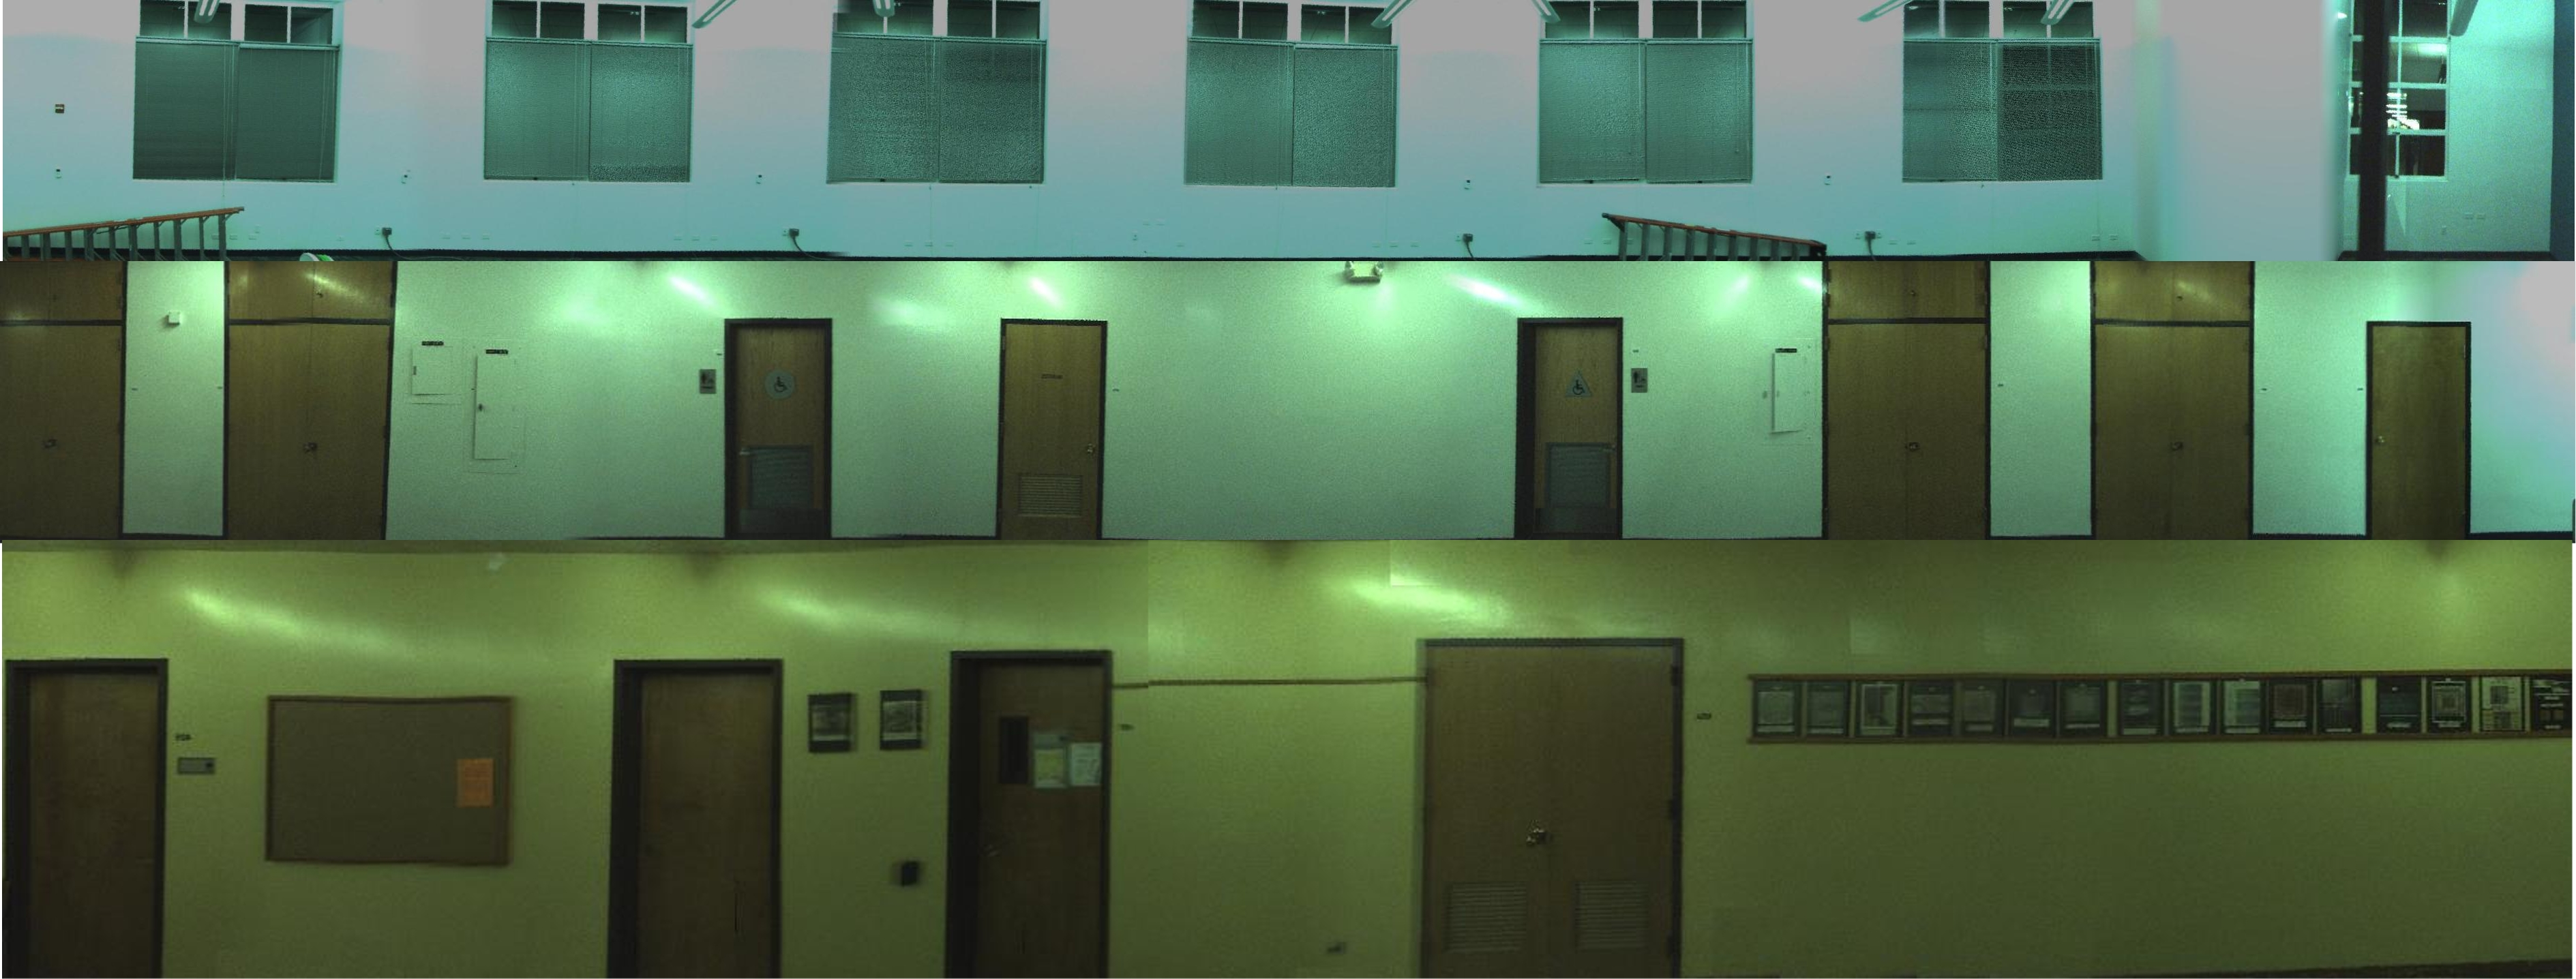
\includegraphics[width=3in]{finalfloors.jpg}}
  ~~~~~~
  \centering
  \subfloat[][]{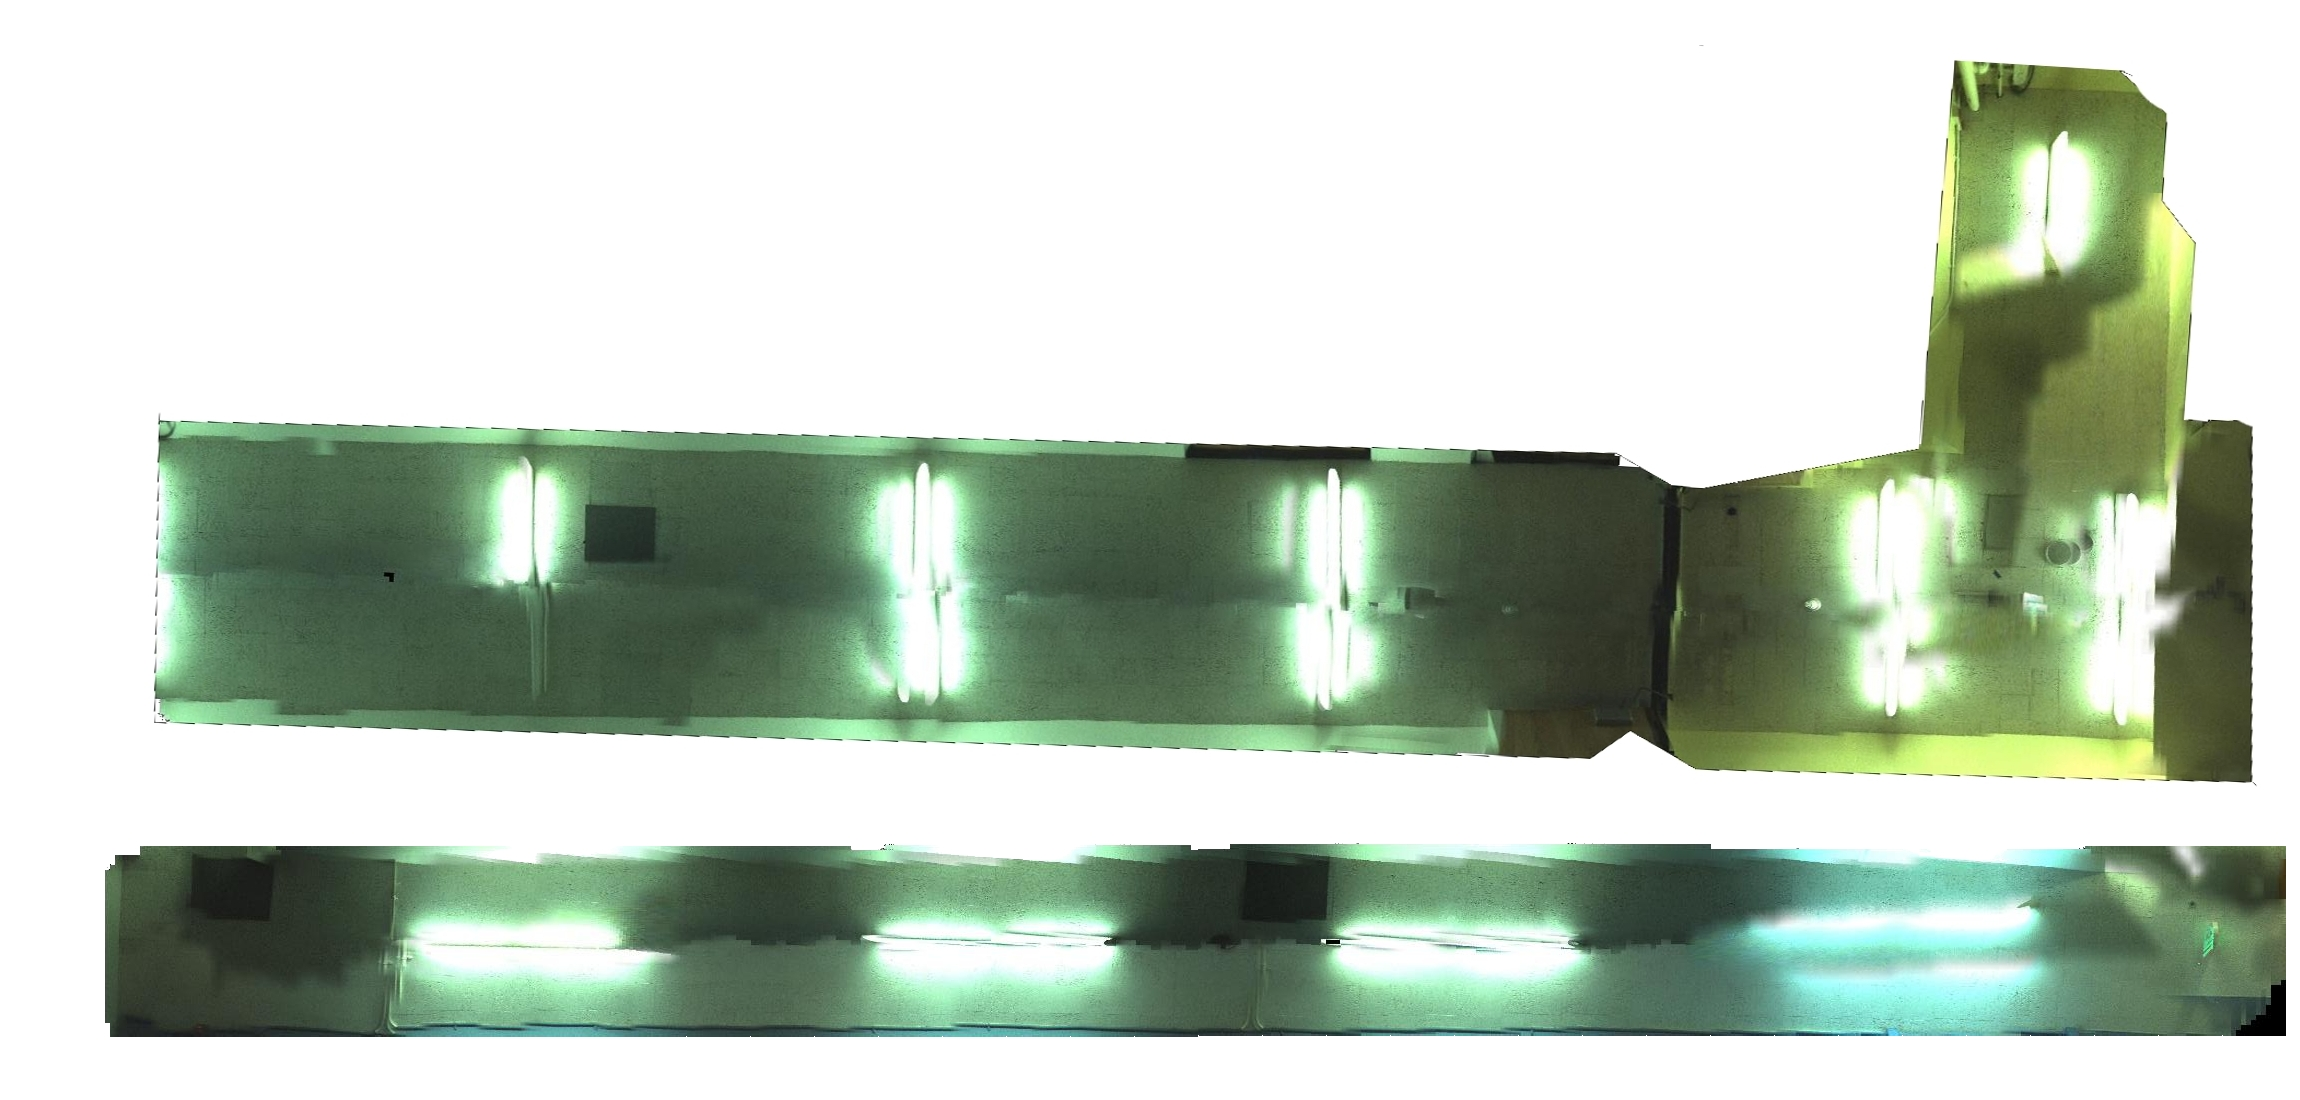
\includegraphics[width=3in]{finalceilings.jpg}}

  \centering
  \subfloat[][]{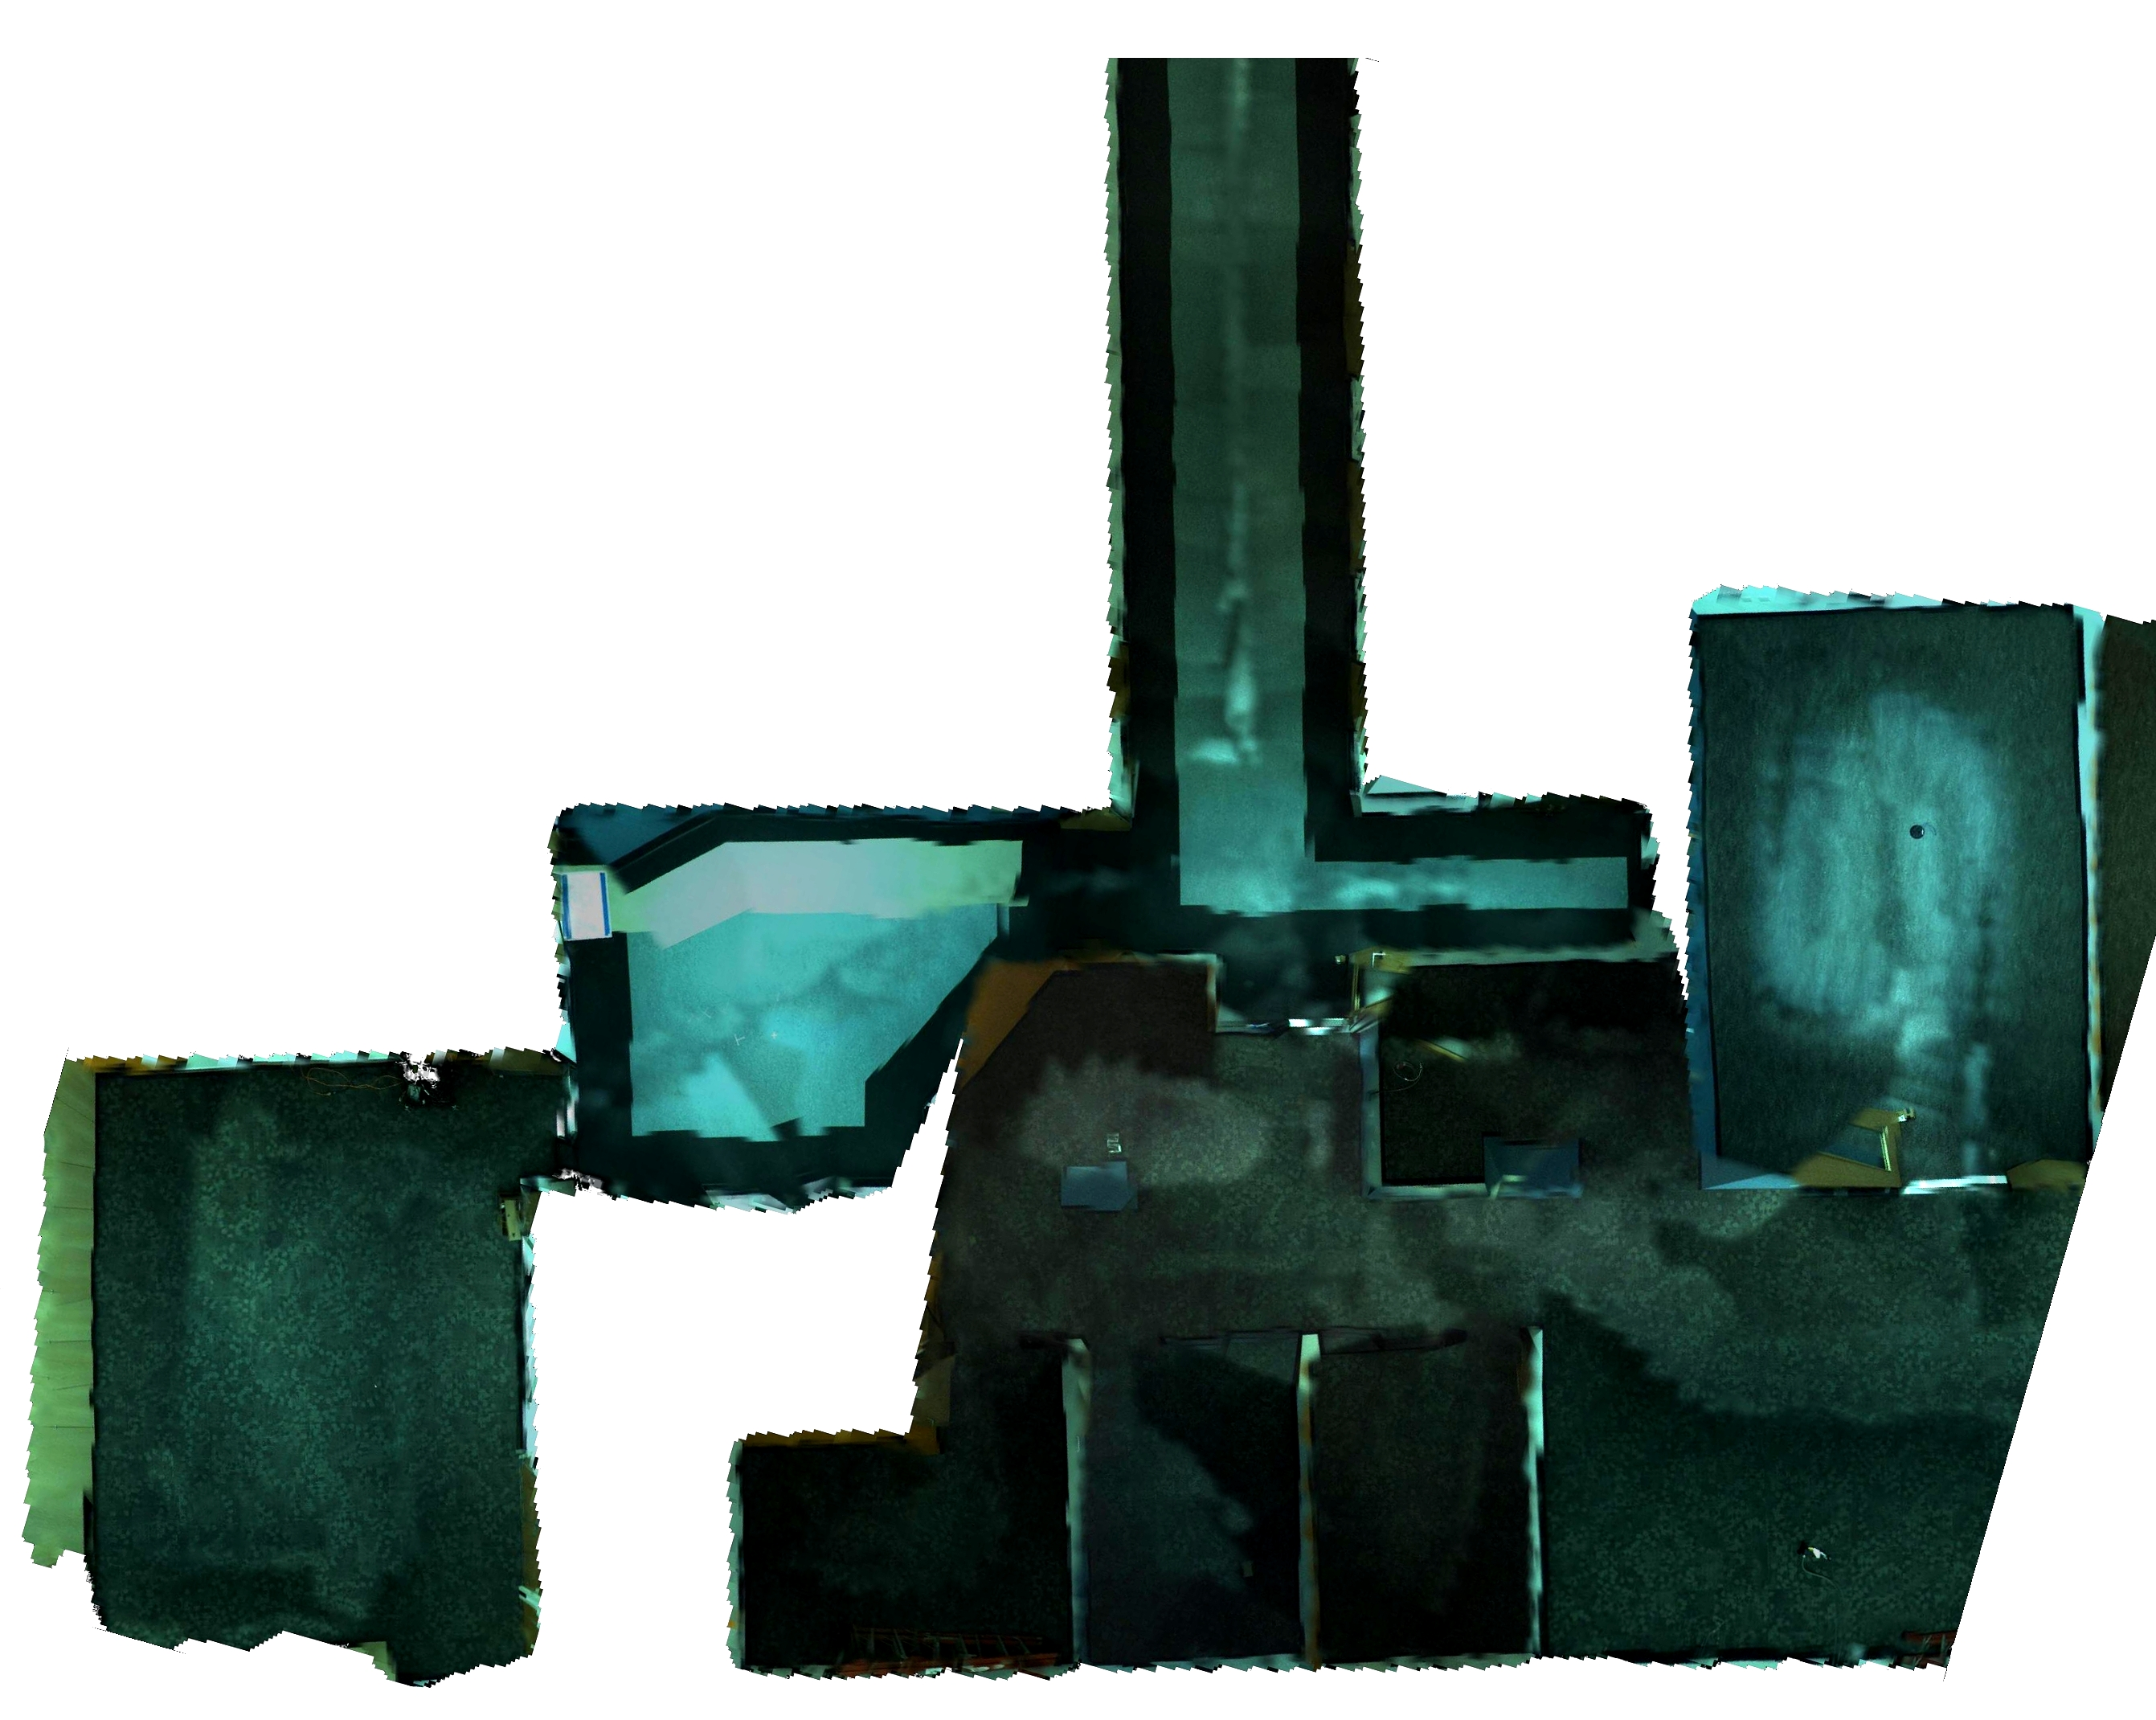
\includegraphics[height=2in, width=3in]{floorcropped.jpg}}
  ~~~~~~~~
  \centering \subfloat[][]{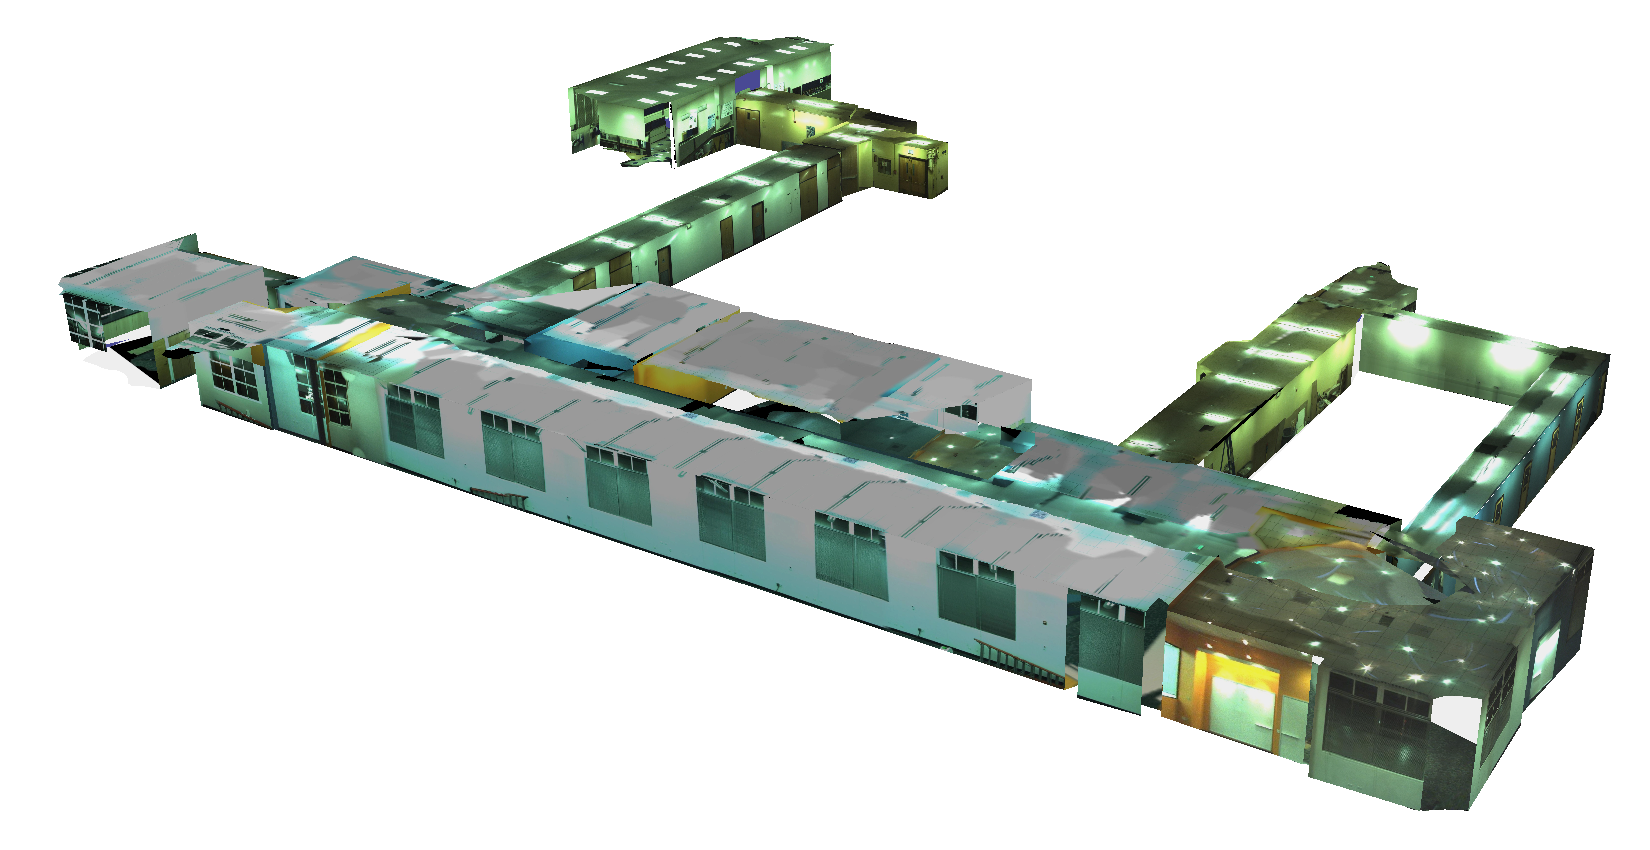
\includegraphics[width=3in]{fullmodel.png}}
  \caption{Examples of our final texture mapping output for (a) walls,
    (b) ceilings, (c) an entire floor, (d) a full model.}
  \label{fig:results}
\end{figure*}

{\small \bibliographystyle{ieee} \bibliography{egbib} }



\message{ !name(oldpaper.tex) !offset(665) }

\end{document}
